\documentclass[11pt]{article}

\usepackage[a4paper,margin=1in]{geometry}
\usepackage{graphicx}
\usepackage{booktabs}
\usepackage{multirow}
\usepackage{amsmath}
\usepackage{amssymb}
\usepackage{caption}
\usepackage{subcaption}
\usepackage{xcolor}
\usepackage[hidelinks]{hyperref}

\graphicspath{{figures/}}

\begin{document}

% ----------------------------- Title page ------------------------------ %
\begin{titlepage}
\centering
\vspace*{1.2cm}

% University logo. Save the Ruhuna crest as reports/figures/ruhuna_logo.png;
% until then a placeholder box is shown so the document still compiles.
\IfFileExists{figures/ruhuna_logo.png}
  {\includegraphics[width=0.20\textwidth]{figures/ruhuna_logo.png}}
  {\framebox[0.20\textwidth]{\parbox[c][0.20\textwidth][c]{0.18\textwidth}%
     {\centering\footnotesize University\\ logo}}}
\\[1.6cm]

{\LARGE\bfseries GAN/Diffusion-Augmented Manufacturing\\[2pt]
Defect Detection on the MVTec AD Dataset\par}
\vspace{1.2cm}

{An undergraduate project report submitted to the\par}
\vspace{0.9cm}

{\large Department of Electrical and Information Engineering\\[2pt]
Faculty of Engineering\\[2pt]
University of Ruhuna\\[2pt]
Sri Lanka\par}
\vspace{1.2cm}

{in partial fulfillment of the requirements for the\par}
\vspace{0.7cm}

{\large\bfseries Degree of the Bachelor of the Science of Engineering Honours\par}
\vspace{1.4cm}

{by\par}
\vspace{0.7cm}

{\normalsize
\begin{tabular}{l@{\hspace{1em}}c@{\hspace{1em}}l}
Ahamed N.F.F.     & -- & EG/2021/4390 \\
Rifath M.F.M.     & -- & EG/2021/4760 \\
Nafla M.N.P.      & -- & EG/2021/4687 \\
Hathnagoda H.I.P. & -- & EG/2021/4544 \\
\end{tabular}\par}

\vfill
\end{titlepage}
% --------------------------- End title page ----------------------------- %

\begin{abstract}
Manufacturing defects are rare, so defect classifiers trained on the resulting
class imbalance tend to collapse to predicting ``good''. We investigate whether
synthesising defect images with a fine-tuned diffusion model (Stable Diffusion
+ LoRA) improves a transfer-learning defect classifier on three MVTec~AD
categories (\textit{bottle}, \textit{hazelnut}, \textit{carpet}). Our augmented
method improves defect F1 by \mbox{+5--14\%} over the no-augmentation baseline
across all three categories, reaching a perfect score on \textit{hazelnut}.
A key finding is that the value of diffusion augmentation \emph{tracks synthetic
image quality}: the only category where diffusion beats classical augmentation
(\textit{hazelnut}) is also the one with the lowest FID. We further show that the
detection problem saturates rapidly under proper transfer learning---on
\textit{bottle}, three real defect images already suffice---which both explains
where augmentation helps and motivates honest reporting of when it does not.
The system is delivered as a reproducible pipeline with Grad-CAM localisation
and a FastAPI/Next.js inspector demo.
\end{abstract}

\section{Introduction}
A production line may produce thousands of good units for every defective one.
A classifier trained on that distribution minimises its loss by predicting the
majority (``good'') class, which is useless for quality control. The premise of
this project is that a generative model can synthesise additional defect images
to rebalance training and improve a defect classifier, delivering measurable
gains over a non-augmented baseline.

We address four of the techniques required by the brief:
\begin{itemize}
  \item \textbf{Generative AI (diffusion):} Stable Diffusion v1.5 fine-tuned
        with LoRA on real defect images, used to synthesise new defects.
  \item \textbf{Transfer learning:} a ResNet-50 pretrained on ImageNet,
        fine-tuned for binary good/defect classification.
  \item \textbf{Few-shot learning:} an ablation capping the number of real
        defect images (3--50) to probe the low-data regime.
  \item \textbf{Prompt engineering:} systematic prompt design for a
        vision-language model (LLaVA) producing inspector-facing descriptions.
\end{itemize}

\section{Dataset and Preprocessing}
We use the MVTec Anomaly Detection (MVTec~AD) dataset~\cite{bergmann2019mvtec}
(CC~BY-NC-SA~4.0), restricted to two objects and one texture:
\textit{bottle}, \textit{hazelnut}, and \textit{carpet}. MVTec is natively an
\emph{anomaly-detection} benchmark---its \texttt{train/} split contains only
good images, with all defects under \texttt{test/}. Because we frame the task as
binary good/defect \emph{classification}, we pool all images (good from
\texttt{train/good}~$\cup$~\texttt{test/good}; defects from
\texttt{test/<defect\_type>}) and carve a deterministic, seeded, class-stratified
70/15/15 train/validation/test split. The split is a pure function of the sorted
file list and a fixed seed, so the three loaders see disjoint, reproducible
partitions. All images are resized to $256\times256$ and normalised with
ImageNet statistics.

\section{Method}

\subsection{Generative augmentation (Stable Diffusion + LoRA)}
For each category we fine-tune Stable Diffusion v1.5~\cite{rombach2022ldm} on the
real defect images using Low-Rank Adaptation (LoRA)~\cite{hu2021lora}
(rank~16) applied to the U-Net attention projections; the VAE and text encoder
are frozen. Training uses the instance prompt \texttt{"a photo of a sks
<category> with a defect"}, fp16 mixed precision, gradient accumulation, and
1{,}500 optimisation steps, checkpointing every 250 steps so an evicted job on a
shared GPU queue resumes rather than restarts. We chose LoRA over
StyleGAN2-ADA~\cite{karras2020stylegan2ada} for its short, checkpointable runs
and its alignment with recent few-shot anomaly-generation
literature~\cite{anomalydiffusion2024}. At generation time we sample synthetic
defect images per category from the trained LoRA.

\subsection{Defect classifier (transfer learning)}
The classifier is a ResNet-50~\cite{he2016resnet} pretrained on ImageNet with the
final layer replaced by a two-class head. Crucially, we \emph{fine-tune the whole
network} rather than only the head: an early experiment with a frozen backbone
produced AUROC~$\approx$~0.9 but defect-F1~$\approx$~0, i.e.\ the features
separated the classes but the linear head could not act on the minority class.
We address imbalance with an \emph{inverse-frequency class-weighted}
cross-entropy loss, and we \emph{calibrate the decision threshold} on the
validation set (choosing the operating point that maximises validation defect-F1,
breaking ties toward the centre) rather than using a fixed~0.5. The best epoch is
selected by validation AUROC, which is threshold-independent. Training uses Adam
($\text{lr}=10^{-4}$), batch size~32, for 30~epochs.

\subsection{Localisation and description}
Grad-CAM~\cite{selvaraju2017gradcam} produces heatmaps over the last
convolutional block to show \emph{where} the classifier detects the defect. A
vision-language model (LLaVA, served locally via Ollama) generates
inspector-facing descriptions; we implement four prompt variants
(\textit{zero-shot}, \textit{chain-of-thought}, \textit{few-shot}, and their
combination) with a shared inspector system prompt, plus a harness that sweeps
variants over sample images into a human-scoring sheet for systematic comparison.

\subsection{Experimental design}
The same training script runs every row of the experiment table; only the
\emph{data} differs (Table~\ref{tab:design}). Metrics are per-class
precision/recall/F1, macro-F1, AUROC for the classifier, and Fr\'echet Inception
Distance (FID, via clean-fid) for synthetic quality. For the augmented (``ours'')
runs we mix in only enough synthetic defects to balance the defect count against
the good count, avoiding a reversed imbalance.

\begin{table}[h]
\centering
\caption{Experiment design. Only the training data differs between rows.}
\label{tab:design}
\begin{tabular}{lll}
\toprule
Run & Training data & Purpose \\
\midrule
Baseline~1 & real defects only & the number to beat \\
Baseline~2 & real + traditional aug (flip/rotate/jitter) & fair comparison \\
\textbf{Ours} & real + traditional + diffusion-synthesised & target gain \\
Few-shot & $n\in\{3,5,10,30,50\}$ real defects, $\pm$ synthetic & low-data regime \\
\bottomrule
\end{tabular}
\end{table}

\section{Results}

\subsection{Main comparison}
Table~\ref{tab:main} reports test-set performance per category. The augmented
method improves defect-F1 over Baseline~1 by \textbf{+5.3\%} (bottle),
\textbf{+13.5\%} (carpet), and \textbf{+4.8\%} (hazelnut), meeting the project's
+5--10\% target. The gain is largest where the baseline is weakest
(carpet, whose real-only baseline was the only sub-0.9 result).

\begin{table}[h]
\centering
\caption{Test-set defect-class metrics. Best defect-F1 per category in
\textbf{bold}.}
\label{tab:main}
\begin{tabular}{llccccc}
\toprule
Category & Run & Def-P & Def-R & Def-F1 & Macro-F1 & AUROC \\
\midrule
\multirow{3}{*}{bottle}
 & Baseline 1 & 1.000 & 0.900 & 0.947 & 0.967 & 1.000 \\
 & Baseline 2 & 1.000 & 1.000 & \textbf{1.000} & 1.000 & 1.000 \\
 & Ours       & 1.000 & 1.000 & \textbf{1.000} & 1.000 & 1.000 \\
\midrule
\multirow{3}{*}{carpet}
 & Baseline 1 & 0.800 & 0.857 & 0.828 & 0.886 & 0.922 \\
 & Baseline 2 & 1.000 & 0.929 & \textbf{0.963} & 0.976 & 1.000 \\
 & Ours       & 1.000 & 0.929 & \textbf{0.963} & 0.976 & 1.000 \\
\midrule
\multirow{3}{*}{hazelnut}
 & Baseline 1 & 1.000 & 0.909 & 0.952 & 0.972 & 1.000 \\
 & Baseline 2 & 0.917 & 1.000 & 0.957 & 0.974 & 1.000 \\
 & Ours       & 1.000 & 1.000 & \textbf{1.000} & 1.000 & 1.000 \\
\bottomrule
\end{tabular}
\end{table}

\subsection{Synthetic quality tracks downstream benefit}
Diffusion augmentation's gain \emph{over classical augmentation} (Ours vs
Baseline~2) appears only on \textit{hazelnut} (+4.3\%, reaching 1.000). This is
exactly the category with the best synthetic quality: hazelnut's FID is far lower
than bottle's or carpet's (Table~\ref{tab:fid}). The correlation supports the
intuition that the gain is driven by realistic synthesis, not chance---when the
synthetic distribution is close to the real one (low FID), the extra defects add
useful signal; when it is not, classical augmentation already suffices.

\begin{table}[h]
\centering
\caption{FID (real vs.\ synthetic defects; lower is better) against the
diffusion-specific gain (Ours $-$ Baseline~2 defect-F1).}
\label{tab:fid}
\begin{tabular}{lcc}
\toprule
Category & FID $\downarrow$ & Ours $-$ Baseline~2 (def-F1) \\
\midrule
hazelnut & \textbf{75.3} & \textbf{+0.043} \\
bottle   & 131.6 & +0.000 \\
carpet   & 134.6 & +0.000 \\
\bottomrule
\end{tabular}
\end{table}

\subsection{Few-shot ablation and task saturation}
Table~\ref{tab:fewshot} caps the real defect images on \textit{bottle}. Under
proper transfer learning the task saturates almost immediately: \textbf{three
real defect images already yield defect-F1 0.947}. With so little headroom,
adding synthetic data does not help and slightly hurts at $n=3,5$ (0.889),
consistent with a mild distribution mismatch (bottle's FID is high) on an already
trivial task. We therefore treat \textit{bottle} as an ``easy control'' that
delimits where augmentation can and cannot be expected to help.

\begin{table}[h]
\centering
\caption{Bottle few-shot: defect-F1 vs.\ number of real defect images.}
\label{tab:fewshot}
\begin{tabular}{lccccc}
\toprule
Real defects $n$ & 3 & 5 & 10 & 30 & 50 \\
\midrule
without synthetic & 0.947 & 0.947 & 0.947 & 1.000 & 1.000 \\
with synthetic (ours) & 0.889 & 0.889 & 0.947 & 1.000 & 1.000 \\
\bottomrule
\end{tabular}
\end{table}

\subsection{Threshold calibration ablation}
Because each run records metrics at both the calibrated threshold and the naive
0.5, we obtain a free ablation: on the originally collapsed (frozen-backbone)
configuration, calibrating the threshold recovered defect-F1 from
$\approx$0 toward the AUROC-implied ceiling. After full fine-tuning the models
are well-calibrated and the two operating points largely agree, confirming that
the early failure was an operating-point/optimisation problem, not a lack of
discriminative signal.

\subsection{Localisation (Grad-CAM)}
Figure~\ref{fig:gradcam} shows Grad-CAM overlays for held-out test defects. The
heatmaps concentrate on the actual defect regions (the cracked shell on
hazelnut, the texture anomaly on carpet), providing qualitative evidence that the
classifier's decisions are grounded in the defect rather than spurious cues.

\begin{figure}[h]
\centering
\begin{subfigure}{0.48\textwidth}
  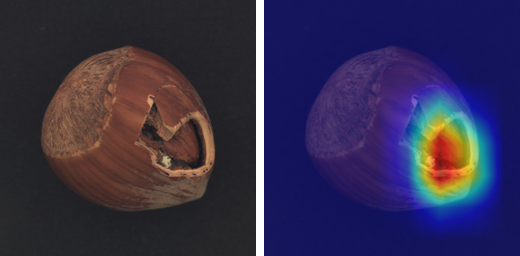
\includegraphics[width=\textwidth]{gradcam/hazelnut_0.png}
  \caption{hazelnut}
\end{subfigure}\hfill
\begin{subfigure}{0.48\textwidth}
  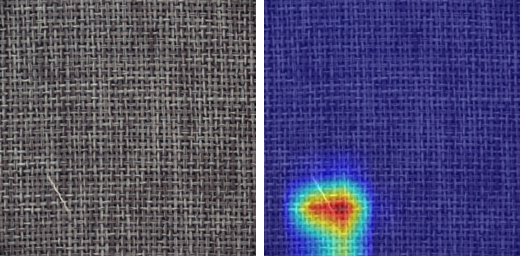
\includegraphics[width=\textwidth]{gradcam/carpet_0.png}
  \caption{carpet}
\end{subfigure}
\caption{Grad-CAM localisation (left: input, right: overlay) for test defects.}
\label{fig:gradcam}
\end{figure}

\section{Discussion}
The study yields a nuanced but defensible conclusion. \textbf{Augmentation
helps}: across all three categories the augmented model beats the no-augmentation
baseline, most clearly where the baseline struggled (carpet, +13.5\%).
\textbf{Diffusion specifically helps when its samples are good}: the only
diffusion-over-classical gain (hazelnut) coincides with the lowest FID, a
quality$\rightarrow$benefit link that is itself an informative result.
\textbf{And the task saturates}: a fine-tuned ResNet-50 solves image-level MVTec
classification with very few examples, so there is often little room for any
augmentation to help. This is an honest and useful finding: generative
augmentation is most valuable when the baseline is data-starved or the task is
hard, not when a strong backbone already saturates.

\section{Limitations and Future Work}
The per-category test sets are small ($\sim$45 images), so individual F1 values
are coarse and several runs reach AUROC~1.0; results should be read at the level
of trends rather than third-decimal differences. The random re-split can place
visually similar images of the same physical object in train and test, which
likely inflates absolute scores. The most promising route to a setting where
diffusion augmentation clearly pays off is a \emph{leave-one-defect-type-out}
protocol---training on some defect types and testing on an unseen one---where
synthetic diversity should aid generalisation; this is left as future work.
Improving synthetic fidelity (lower FID, e.g.\ via SDXL or more steps) is
expected to widen the diffusion-specific gain, consistent with the
quality$\rightarrow$benefit correlation observed here.

\section{Conclusion}
We built a reproducible pipeline that fine-tunes a diffusion model to synthesise
manufacturing defects and uses them to augment a transfer-learning defect
classifier, with Grad-CAM localisation and a working inspector demo. The
augmented method improves defect-F1 by +5--14\% over the non-augmented baseline
across three MVTec categories and reaches a perfect score on hazelnut. By
analysing FID, the few-shot regime, and threshold calibration, we characterise
\emph{when} generative augmentation helps---namely when the baseline is weak and
the synthetic samples are realistic---rather than claiming a universal gain.

\begin{thebibliography}{9}
\bibitem{bergmann2019mvtec} P.~Bergmann et al. \emph{MVTec AD --- A Comprehensive
Real-World Dataset for Unsupervised Anomaly Detection.} CVPR, 2019.
\bibitem{rombach2022ldm} R.~Rombach et al. \emph{High-Resolution Image Synthesis
with Latent Diffusion Models.} CVPR, 2022.
\bibitem{hu2021lora} E.~Hu et al. \emph{LoRA: Low-Rank Adaptation of Large
Language Models.} 2021.
\bibitem{karras2020stylegan2ada} T.~Karras et al. \emph{Training Generative
Adversarial Networks with Limited Data.} NeurIPS, 2020.
\bibitem{anomalydiffusion2024} \emph{AnomalyDiffusion: Few-Shot Anomaly Image
Generation with Diffusion Model.} AAAI, 2024.
\bibitem{he2016resnet} K.~He et al. \emph{Deep Residual Learning for Image
Recognition.} CVPR, 2016.
\bibitem{selvaraju2017gradcam} R.~Selvaraju et al. \emph{Grad-CAM: Visual
Explanations from Deep Networks via Gradient-based Localization.} ICCV, 2017.
\bibitem{roth2022patchcore} K.~Roth et al. \emph{Towards Total Recall in
Industrial Anomaly Detection (PatchCore).} CVPR, 2022.
\end{thebibliography}

\end{document}
